% !TeX root = RJwrapper.tex
\title{R Packages to Aid in Handling Web Access Logs}
\author{by Oliver Keyes, Bob Rudis, Jay Jacobs}

\maketitle

\abstract{%
Web access logs contain information on HTTP(S) requests and form a key
part of both industry and academic explorations of human behaviour on
the internet - explorations commonly performed in R. In this paper we
explain and demonstrate a series of packages designed to efficiently
read in, parse and munge access log data, allowing researchers to handle
it easily.
}

\subsection{Introduction}\label{introduction}

The rise of the World Wide Web over the last few decades has made it
dramatically easier to access and transfer data, and R \citep{RCore}
boasts abundant functionality when it comes to taking data \emph{from}
the web. Base R itself has simple file downloading and page reading
capabilities, through the \texttt{download.file} and \texttt{readLines}
functions, and additional functionality is made available for handling
web-accessible data through packages such as \CRANpkg{httr}
\citep{httr}.

Data \emph{on} the web is not, however, the only kind of web data that
interests researchers; web traffic is, in and of itself, an interesting
data source. Access logs - records of connections between users and a
web server - are an asset and resource for people studying everything
from user behaviour on the internet \citep{halfak}, to website
performance \citep{performance}, to information security
\citep{infosec}.

As a statistically-oriented programming language, R is commonly used by
these same researchers for data analysis, testing and reporting - but it
lacks tools designed for the kinds of data sources and formats that are
encountered when dealing with access logs. In this article we review the
use cases for particular operations over web data, the limitations in
base R when it comes to performing those operations, and a suite of R
packages designed to overcome them: \CRANpkg{webreadr} \citep{webreadr},
designed for reading access logs in, \CRANpkg{urltools}
\citep{urltools}, for URL manipulation, \CRANpkg{iptools}
\citep{iptools} for handling IP addresses, and \CRANpkg{rgeolocate}
\citep{rgeolocate} for direct IP geolocation.

\subsection{Reading access logs}\label{reading-access-logs}

The first task with any data analysis is to read the data into R so that
it can be manipulated. With access logs this is slightly complicated by
the fact that there is no one standard for what a log should look like;
instead, there are multiple competing approaches from different software
platforms and eras. These include the Common Log Format (CLF), the
confusingly-named Combined Log Format, and formats used by individual,
commonly-used software platforms - such as the custom format for the
Squid internet caching software, and the format used by Amazon Web
Services (AWS).

The difference between formats can easily be shown by looking at how
timestamps are represented:

\begin{table}[ht]
\centering
\caption{Timestamps in Common Access Log Formats}
\begin{tabular}{rlr}
  \hline
Log Type & Timestamp Columns & Timestamp Format \\ 
  \hline
Common Log Format & 1 & 10/Oct/2000:13:55:36 -0700\\ 
Combined Log Format & 1 & 26/Apr/2000:00:23:48 -0400\\ 
Squid & 1 & 1286536309.450\\ 
AWS & 2 & 2014-05-23    01:13:11\\ 
   \hline
\end{tabular}
\end{table}

With four log types, we have three different timestamp formats - and
that's only one of the many columns that could appear. These logs also
vary in whether they specify quoting fields (or sanitising unquoted
ones), the columns they contain and the data each column contains in
turn.

To make reading access logs into R as easy as possible we created the
\pkg{webreadr} package. This contains user-friendly equivalents to
\code{read.table} for each type of log, detecting the fields that should
appear, converting the timestamps into POSIX objects, and merging fields
or splitting fields where necessary. The package contains four core
functions, one for each form of log: \code{read\_clf} for the Common Log
Format, \code{read\_combined} for the Combined Log Format, and
\code{read\_squid} and \code{read\_aws} for Squid and AWS formats
respectively. Each one abstracts away the complexity of specifying
column names and formats, and instead allows a researcher to read a file
in with a minimal amount of work.

As the name suggests, it is built not on top of base R but on top of the
\CRANpkg{readr} \citep{readr} package, allowing us to take advantage of
substantial speed improvements that package's base functions have over
base R. These improvements can be seen in the visualisation below, which
uses \CRANpkg{microbenchmark} \citep{microbenchmark} to compare 100
reads of a 600,000-line ``squid'' formatted file with webreadr to the
same operation performed in base R:

\begin{figure}[h]
    \centering
    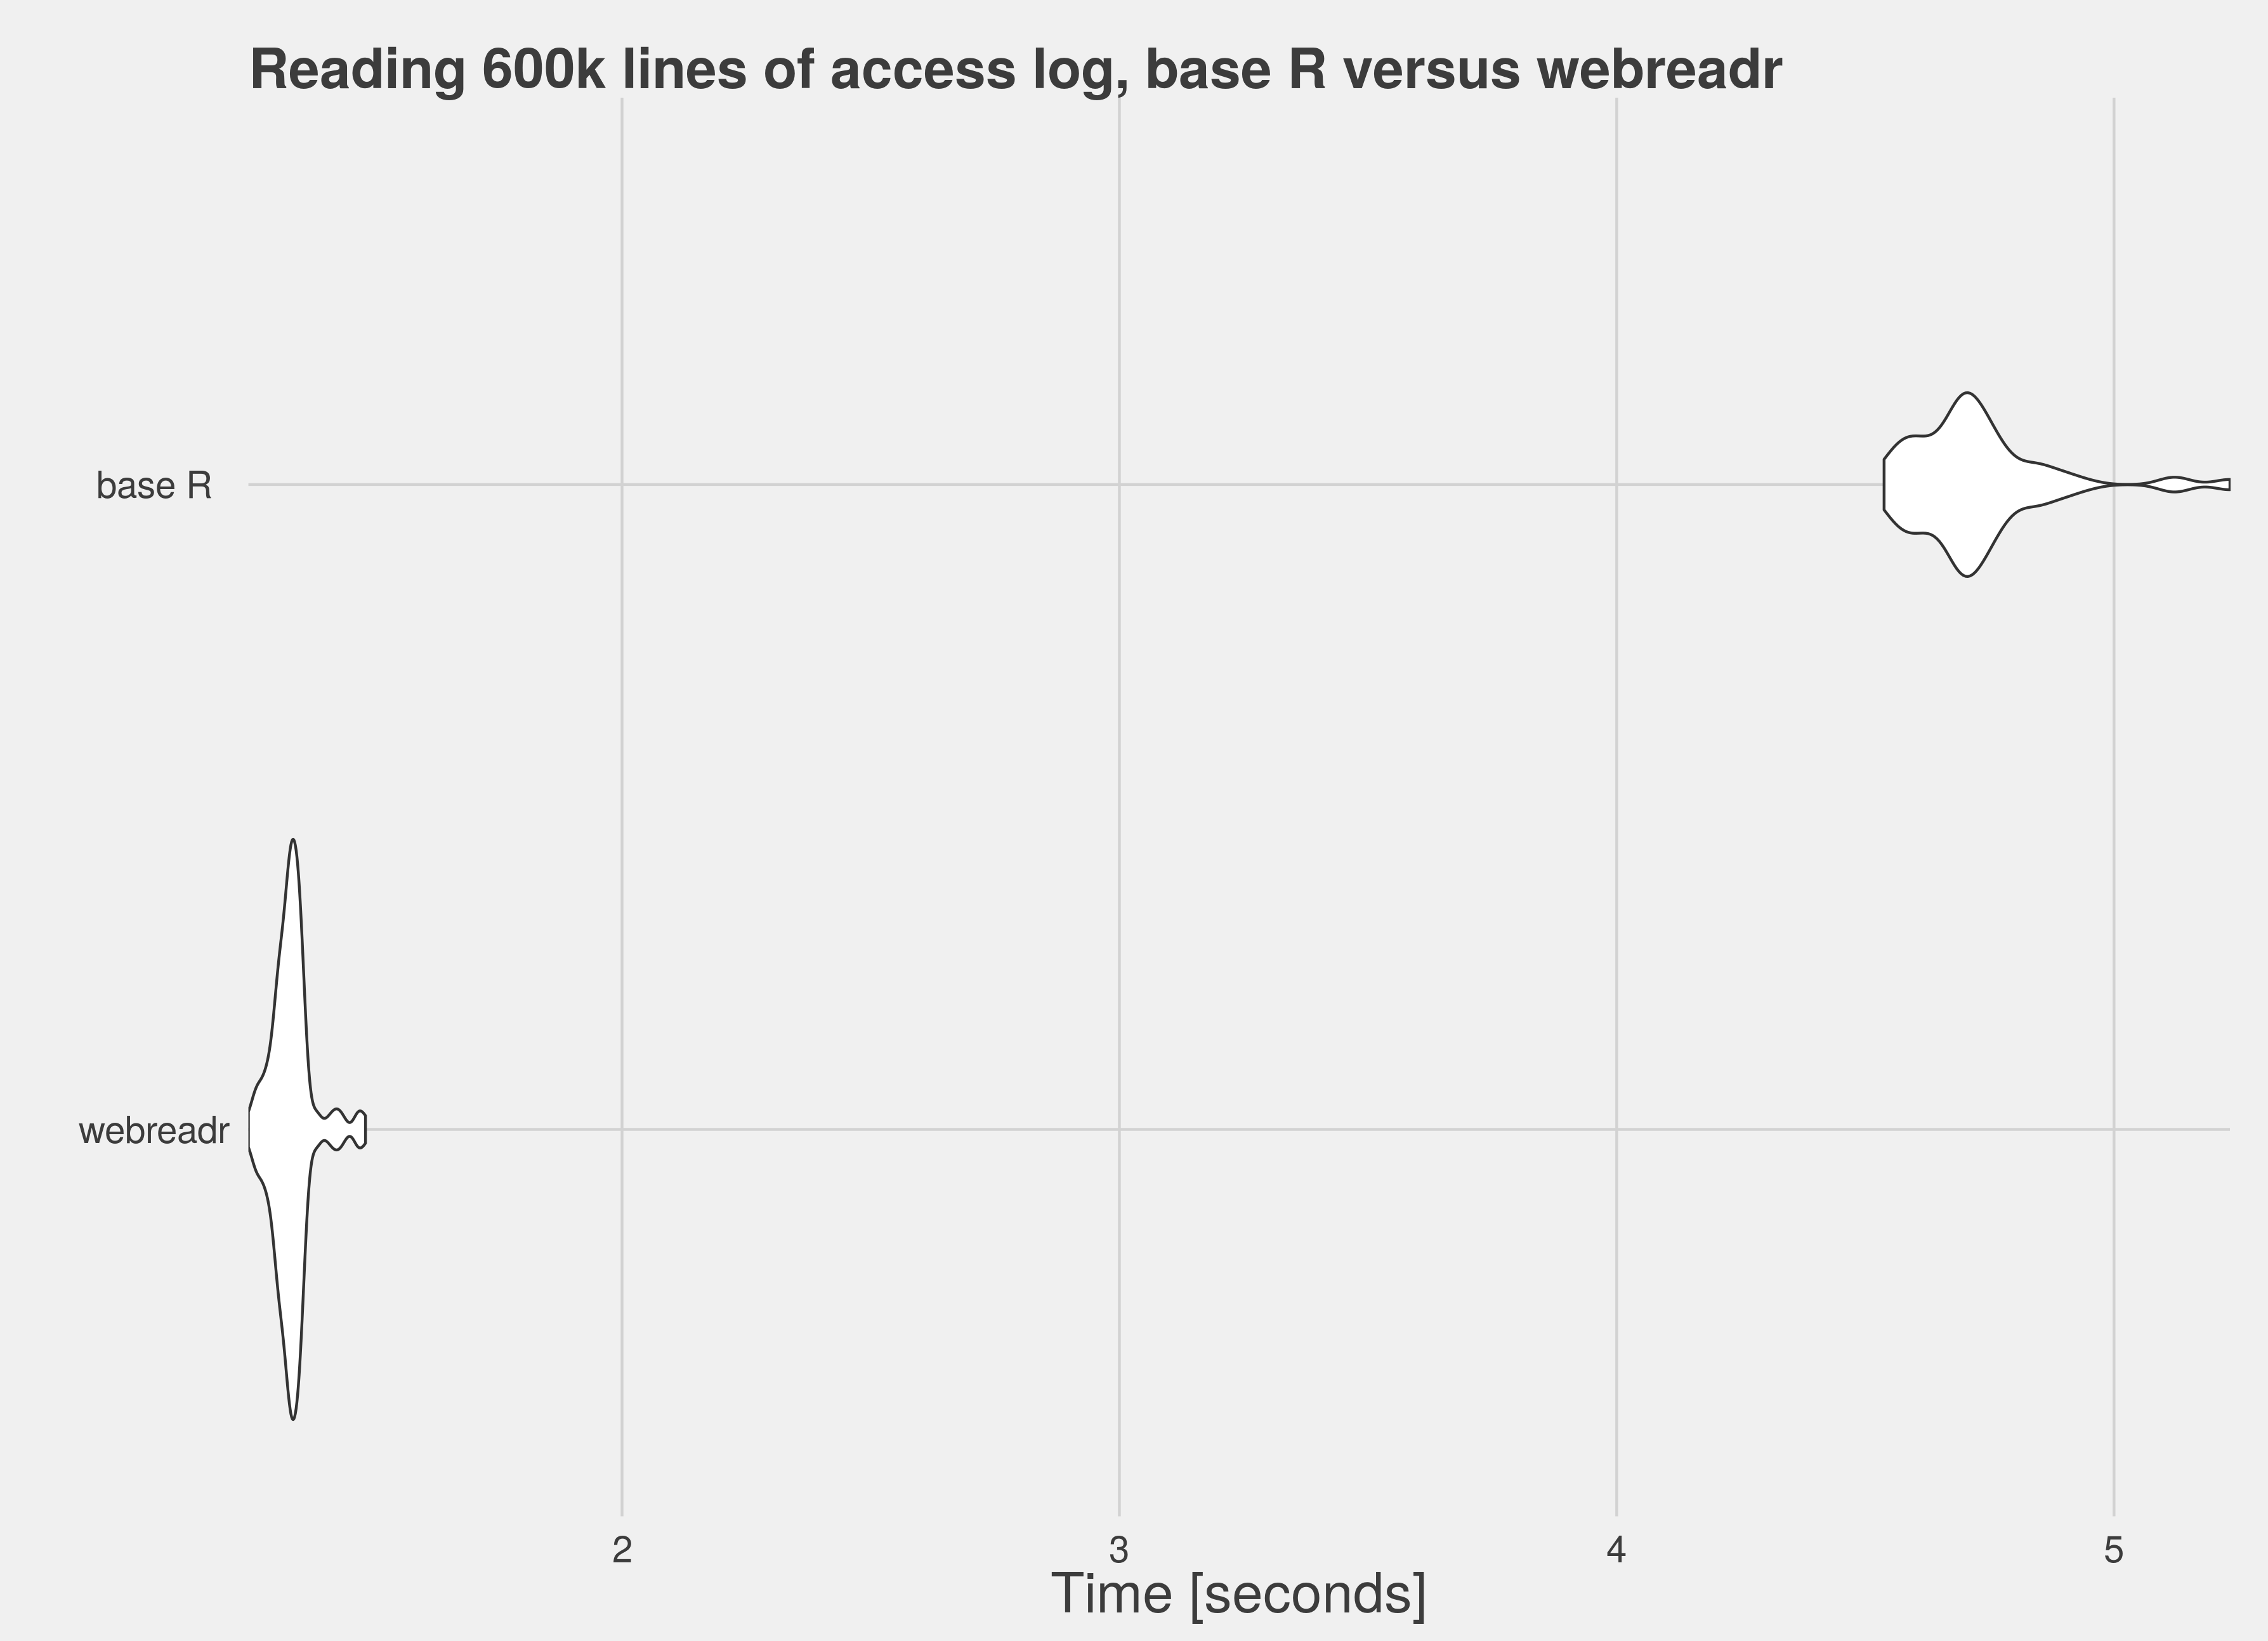
\includegraphics[scale=0.4]{reading_benchmarks}
    \caption{Results of microbenchmark run: read\char`_squid versus base-R equivalent code}
\end{figure}

\pkg{webreadr} takes 1.2 seconds to read this file in at a minimum, and
1.48 at maximum, with a median of 1.33. This is consistently 3.5-6 times
faster than the equivalent base R functionality - and is also, as
explained, far easier to use.

\subsection{Decoding and parsing URLs}\label{decoding-and-parsing-urls}

Within access logs, URLs appear - both to describe the web asset or page
that the user requested and where the user came from. These fields are
usually named url and referer respectively.

\subsubsection{Decoding}\label{decoding}

Both values can be percent-encoded, allowing them toinclude characters
that are valid but reserved by the URL specification as having special
meanings (``reserved characters''). A \samp{\#} symbol, for example, is
encoded as \samp{\%23}: a percentage symbol, followed by the byte-code
for that character.

The encoding of reserved characters is useful, since it means that URL
paths and queries can contain a vast array of values - but it makes data
analysis tougher to do. Examples of common data analysis or cleaning
operations that become more difficult are:

\begin{enumerate}
\def\labelenumi{\arabic{enumi}.}
\itemsep1pt\parskip0pt\parsep0pt
\item
  \textbf{Aggregation}. Aggregating URLs together is useful to identify,
  for example, the relative usage and popularity of particular pages in
  your data - but it becomes tougher if encoding is inconsistent,
  because two URLs could hold the same value but \emph{look} very
  different.
\item
  \textbf{Value selection}. With text-based data, regular expressions
  are a common way of filtering or selecting entries that meet
  particular conditions, but things become fuzzy when you have to look
  not just for particular characters (a space, say) but also the encoded
  values (\%20).
\item
  \textbf{Exploratory data analysis} (EDA). EDA is a common initial step
  to investigate a data set, examining the variables and values it
  contains and whether they meet a researcher's expectations - but on a
  practical basis it becomes difficult when the values aren't
  human-readable.
\end{enumerate}

The solution is to be able to consistently decode URLs, which makes
URL-based data far easier to analyse. Base R does contain a function,
\code{URLdecode}, for doing just that, but is neither vectorised nor
based on compiled code; with large datasets it takes an extremely long
time.

To solve this common problem in analysing request logs, the
\pkg{urltools} package was created. This contains a function,
\code{url\_decode}, which decodes URLs - but relies on vectorised,
compiled code. Benchmarking the two approaches against each other shows
that the \pkg{urltools} implementation is approximately 60-70 times
faster over large datasets. Again using \pkg{microbenchmark}, if we
compare the vectorised decoding of 1,000,000 URLs with \pkg{urltools}
against \code{URLdecode} in a \code{vapply} loop, we see a 60-70 times
speed improvement:

\begin{figure}[h]
    \centering
    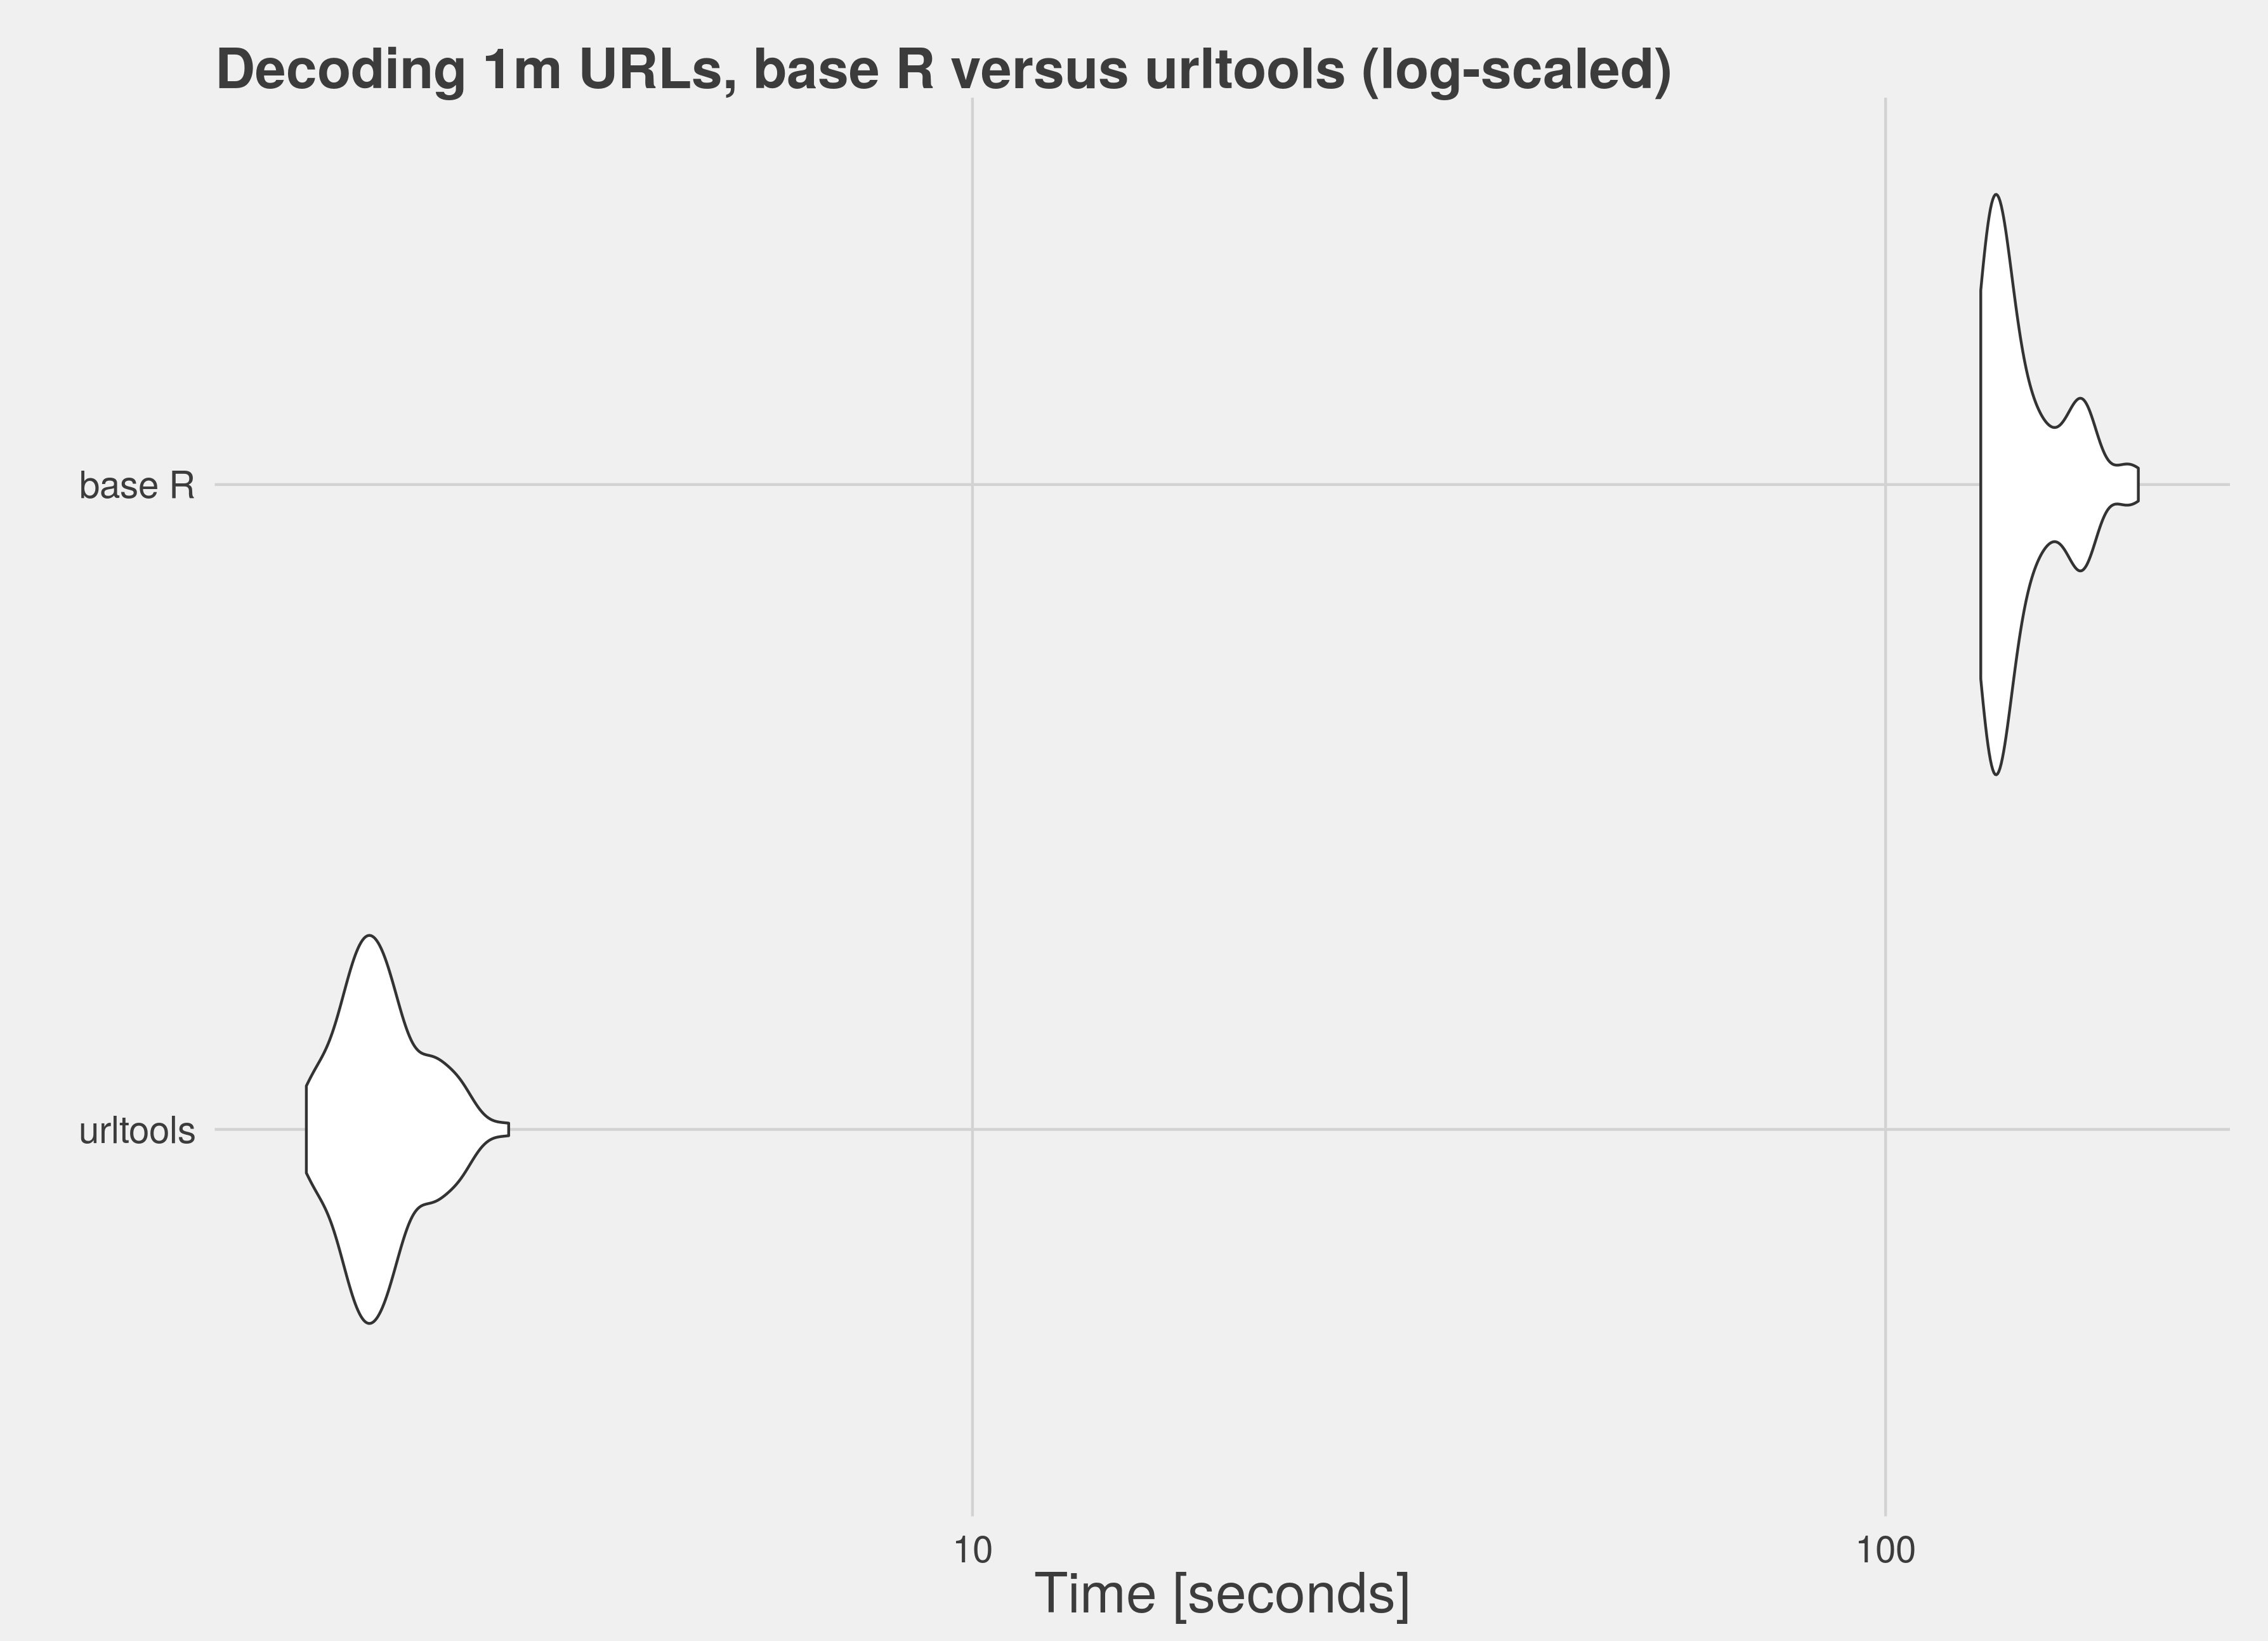
\includegraphics[scale=0.4]{decoding_benchmarks}
    \caption{Results of microbenchmark run: \code{url\_decode} versus base-R equivalent code}
\end{figure}

\subsubsection{Parsing}\label{parsing}

The standard for URLs \citep{RFC1738} divides them into a heirarchical
sequence of components - the scheme (\samp{http}), host
(\samp{en.wikipedia.org}), port (\samp{800}), path
(\samp{wiki/Main\_Page}) and searchpart, or parameters
(\samp{action=edit}). Together, these make up a URL
\linebreak (\samp{http://en.wikipedia.org:800/wiki/Main\_Page?action=edit}).

Parsing URLs to isolate and extract these components is a useful ability
when it comes to exploring request logs; it lets a researcher pick out
particular schemes, paths, hosts or other components to aggregate by,
identifying how users are behaving and what they are visiting. It makes
anonymising data - by removing, for example, the parameters or path,
which can contain relatively unique information - easier.

Base R does not have native code to parse URLs, but the \CRANpkg{httr}
package \citep{httr} contains a function, \code{parse\_url}, designed to
do just that. Built on R's regular expressions, this function is not
vectorised, does not make use of compiled code internally, and produces
a list rather than data.frame, making looping over a set of URLs to
parse each one a time-consuming and awkward experience. This is
understandable given the intent behind that function, which is to
decompose individual URLs within the context of making HTTP requests,
rather than to analyse URLs \emph{en masse}.

\pkg{urltools} contains \code{url_parse} - which does the same thing as
the equivalent \pkg{httr} functionality, but in a vectorised way,
relying on compiled code, and producing a data.frame. Within the context
of parsing and processing access logs, this is far more useful, because
it works efficiently over large sets: httr's functionality, which was
never designed with vectorisation in mind, does not. Indeed,
benchmarking showed that \code{url\_parse} is approximately 570 times
faster than httr's equivalent function:

\begin{figure}[h]
    \centering
    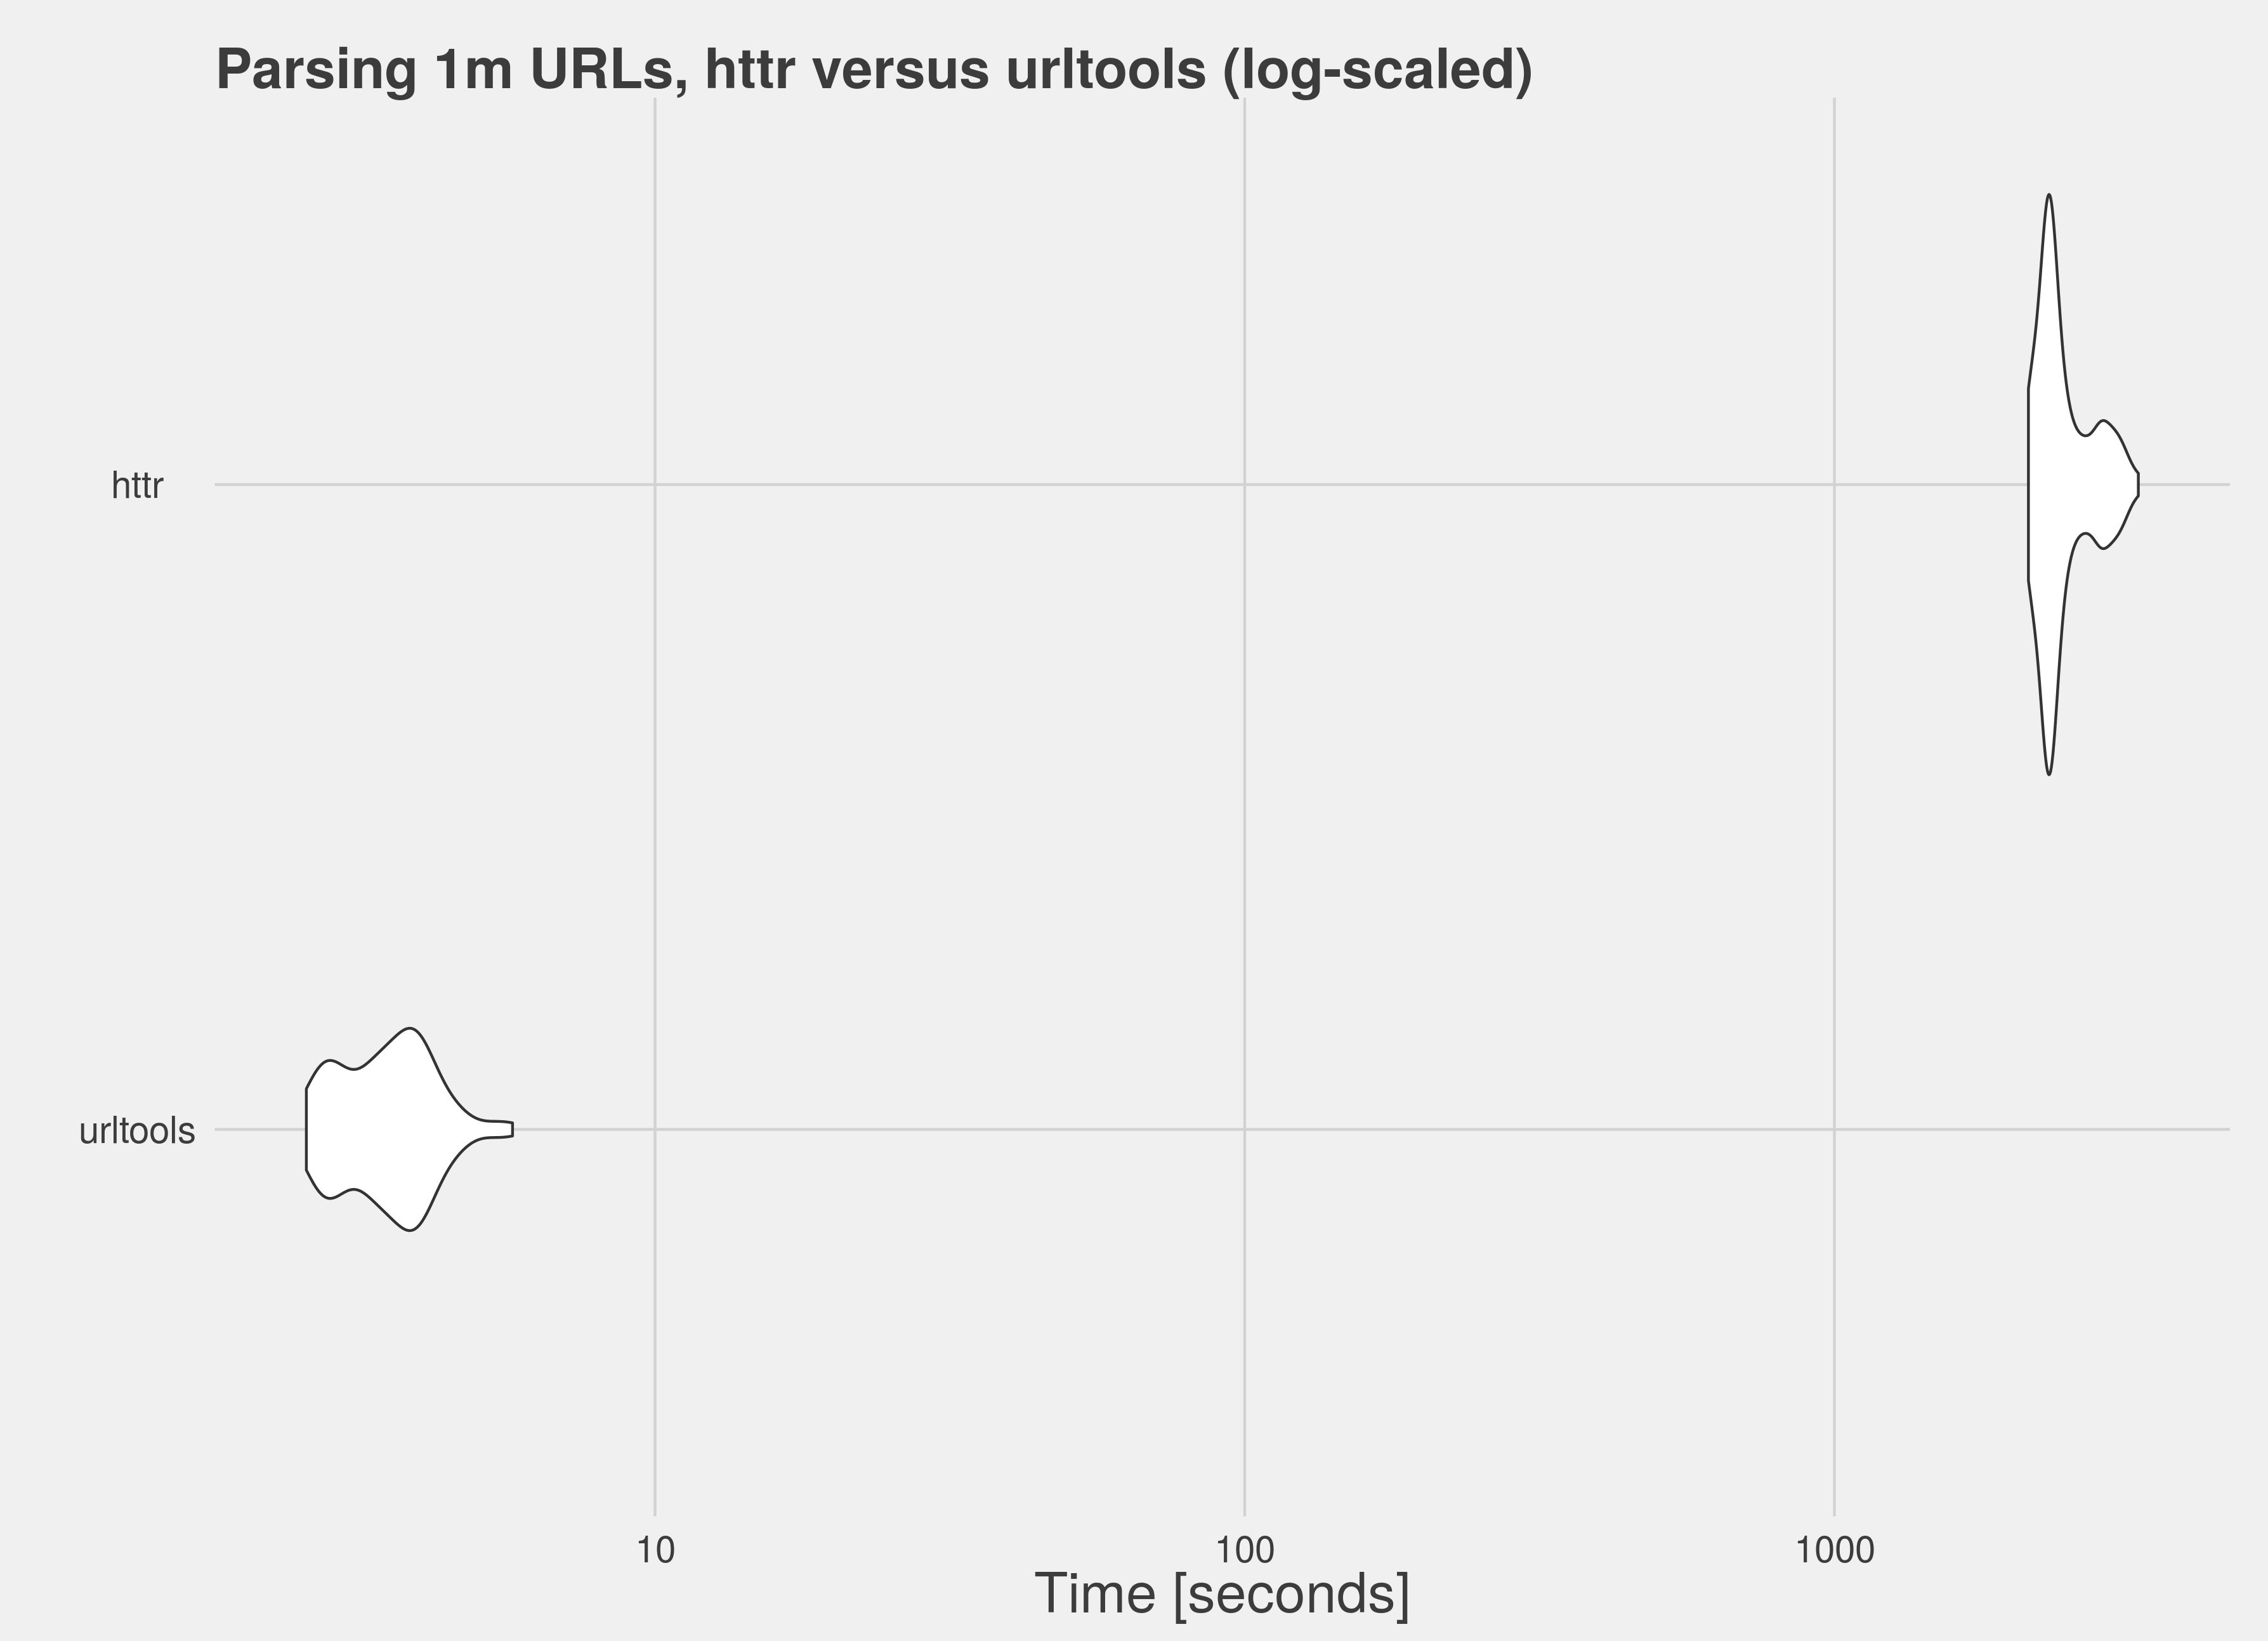
\includegraphics[scale=0.4]{parsing_benchmarks}
    \caption{Results of microbenchmark run: \code{url\_parse} versus httr's equivalent code}
\end{figure}

\newpage

A vector of URLs passed into \texttt{url\_parse} produces a data.frame,
with one column for each of the IETF-supported components, and empty
strings representing components that could not be found. Additionally,
influenced by the style of the \emph{lubridate} package
\citep{lubridate}, \texttt{urltools} contains functions to get or
\emph{set} individual components:

\begin{Schunk}
\begin{Sinput}
# Load urltools and construct a URL
library(urltools)
url <- "http://www.google.com/"

# Get the scheme
scheme(url)
\end{Sinput}
\begin{Soutput}
#> [1] "http"
\end{Soutput}
\end{Schunk}

\begin{Schunk}
\begin{Sinput}
# Set the scheme and observe the modification to the resulting URL
scheme(url) <- "https"
url
\end{Sinput}
\begin{Soutput}
#> [1] "https://www.google.com/"
\end{Soutput}
\end{Schunk}

As a result of this functionality, urltools provides a package to make
URL manipulation faster, easier and far more accessible, reducing the
burden associated with munging access logs or similar datasets and
allowing a researcher to get to the statistical analysis faster.

\subsection{IP manipulation and
geolocation}\label{ip-manipulation-and-geolocation}

Access logs also contain IP addresses - unique numeric values that
identify a particular computer or network in the context of the
internet.

As a side-effect of how IP addresses tend to be assigned - in geographic
blocks, to individual machines or to local networks - they can be used
to geolocate requests, identifying where in the world the request came
from, sometimes down to the level of individual post codes or pairs of
latitude/longitude coordinates.

This is tremendously useful in industry, where the geographic reach of a
service has substantial implications for its viability and
survivability, and in academia, where the locality of internet-provided
information and the breadth of internet access are active concerns and
areas of study \citep{barriers}.

Many services and databases exist for extracting geographic metadata
from IP addresses. One of the most common is the service provided by
MaxMind, which has both proprietary and openly-licensed databases, in
binary and comma-separated formats. The free databases have been used by
various web APIs, which makes the data they contain accessible from R.
Unfortunately, dependence on web APIs means that handling large numbers
of IP addresses can be very slow (they tend to be designed to only
accept one IP address at a time, and may contain throttling beyond that)
and has privacy concerns, since it essentially means sending user IP
addresses to a third party. And even without these issues, there are no
convenient wrappers for those APIs available on CRAN: users have to
hand-roll their own.

With these concerns in mind, we wrote the \CRANpkg{rgeolocate} package.
Through \pkg{httr} this contains convenient, vectorised bindings to
various web services that provide geographic metadata about IP
addresses. More importantly, using the \CRANpkg{Rcpp} package to
integrate C++ and R, \pkg{rgeolocate} also features a direct, compiled
binding to the MaxMind API. This means that local binary databases can
also be queried, which is far faster and more robust than web-based
equivalents and avoids the privacy concerns associated with transmitting
users' IP addresses externally.

The MaxMind API requires a paid or free binary database - one of which,
for country-level IP resolution, is included in \pkg{rgeolocate} - and
allows you to retrieve the continent, country name or ISO code, region
or city name, tzdata-compatible timezone, longitude, latitude or
connection type of a particular IP address. Multiple fields can be
selected (although which are available depends on the type of database
used), and results are returned in a data.frame:

\begin{Schunk}
\begin{Sinput}
# Load rgeolocate
library(rgeolocate)

# Find the rgeolocate-provided binary database
geo_file <- system.file("extdata","GeoLite2-Country.mmdb", package = "rgeolocate")

# Put together some example IP addresses
ip_addresses <- c("174.62.175.82", "196.200.60.51")

# Geolocate
rgeolocate::maxmind(ip_addresses, geo_file, fields = c("continent_name", "country_code"))
\end{Sinput}
\begin{Soutput}
#>   continent_name country_code
#> 1  North America           US
#> 2         Africa           ML
\end{Soutput}
\end{Schunk}

Direct speed comparisons aren't possible, since the functionality it
provides is not (to the authors' knowledge) replicated in other R
packages, but it is certainly faster (and more secure) than
internet-dependent alternatives.

\subsection{Conclusions and further
work}\label{conclusions-and-further-work}

In this research article we have demonstrated a set of tools for
handling access logs during every stage of the data cleaning pipeline -
reading them in with \pkg{webreadr}, decoding, manipulating and
extracting value from URLs with \pkg{urltools}, and retrieving
geographic metadata from IP addresses with \pkg{iptools} and
\pkg{rgeolocate}. We have also demonstrated the dramatic speed
improvements in using these tools in preference to existing methods
within R.

Further work - integrating more sources of geolocation information
within \pkg{rgeolocate}, supporting UTF-8 URL decoding within
\pkg{urltools}, and increasing IPv6 support in \pkg{iptools} - would
make these packages even more useful to Human-Computer Interaction
researchers and other specialists who rely on access logs as primary
data sources. Even without that functionality, however, this suite of
packages is a dramatic improvement upon the status quo.

\bibliography{RJreferences}

\address{%
Oliver Keyes\\
Wikimedia Foundation\\
line 1\\ line 2\\
}
\href{mailto:author1@work}{\nolinkurl{author1@work}}

\address{%
Bob Rudis\\
Rapid7\\
line 1\\ line 2\\
}
\href{mailto:author2@work}{\nolinkurl{author2@work}}

\address{%
Jay Jacobs\\
Magical Python Land\\
line 1\\ line 2\\
}
\href{mailto:author3@work}{\nolinkurl{author3@work}}

